%%%%%%%%%%%%%%%%%%%
% SECTION: LSTM
%%%%%%%%%%%%%%%%%%%
\subsection{Long Short-Term Memory}

Long Short Term Memory networks (LSTM), first introduced by Hochreiter and Schmidhuber \cite{Hochreiter1997LONGMEMORY}, solved the problem of long-term dependencies. These special kind of RNNs are capable of learning both short-term and long-term dependencies although they are specialised for long-term relationships.

% FIGURE: LSTM cell
\begin{figure}[!htb]	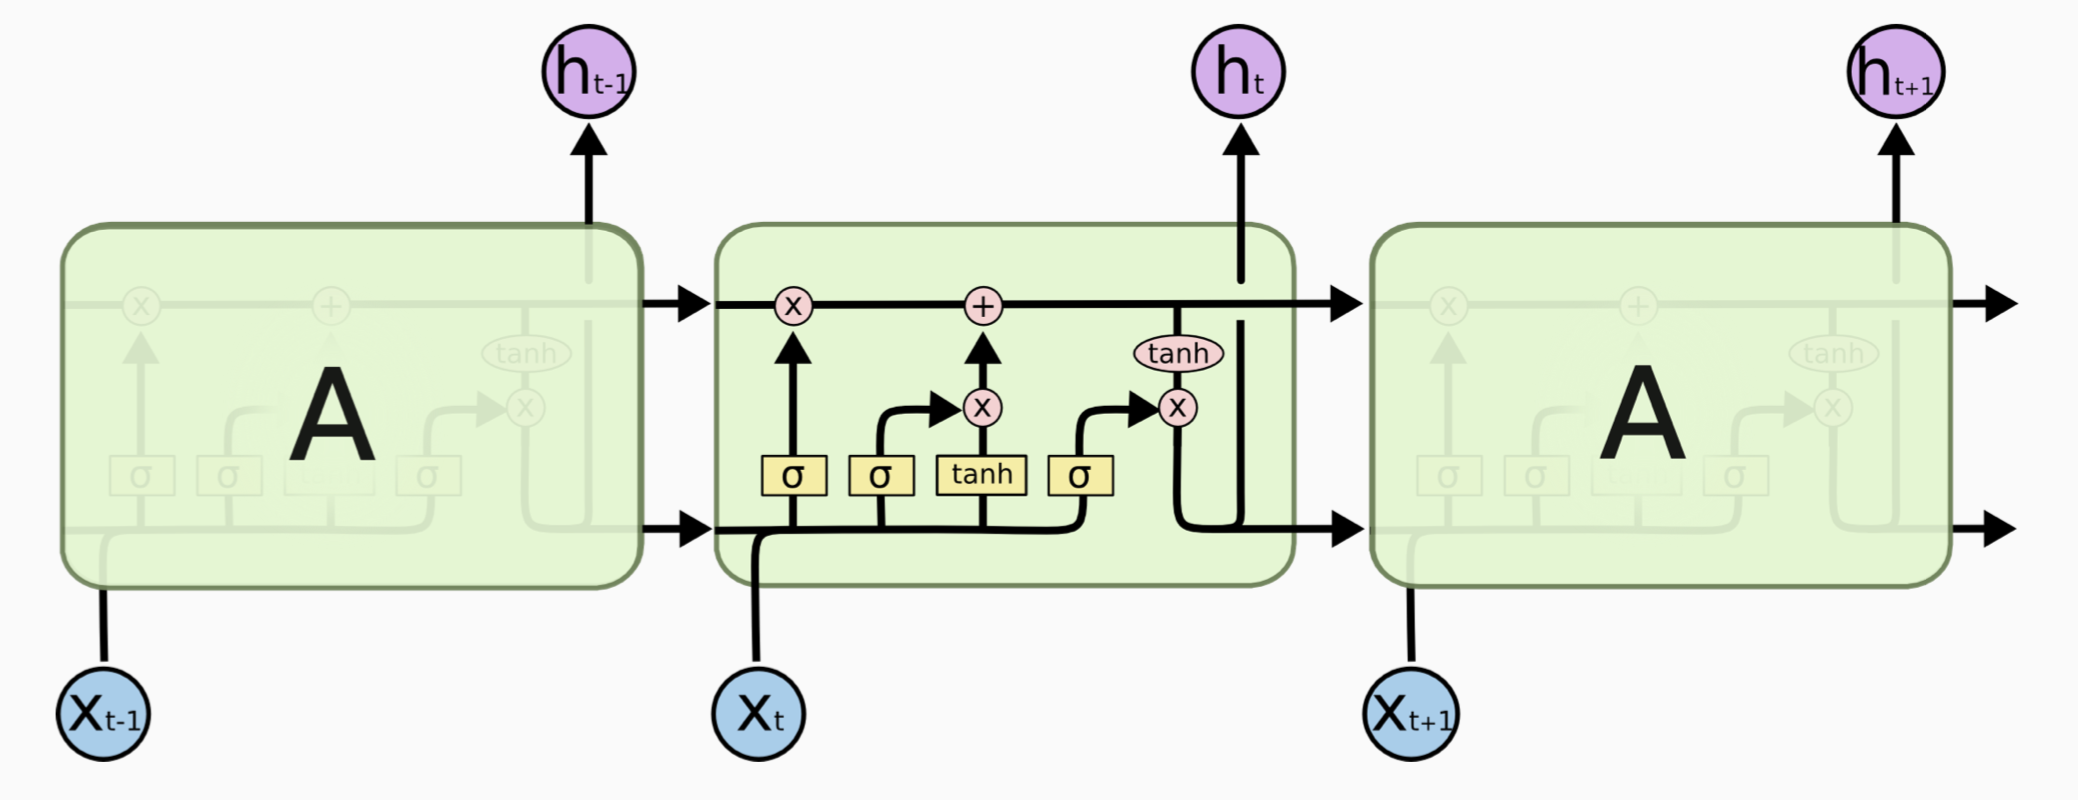
\includegraphics[width=0.9\textwidth]{images/lstm_cell.png} 
    \centering

\caption{
LSTM memory cell and control gates. \cite{OlahChristopher2015UnderstandingNetworks}
} 

\label{fig:LSTM cell}
\end{figure}

An LSTM uses a memory cell in place of a neuron. The memory cell regularise how the information changes from state to state. This gives the LSTM the ability to control how much information should be added or removed from the cell state which is regulated by some gates. A memory cell contains the following gates: Forget Gate, Input Gate, Update Gate and Output Gate. The gates have a sigmoid layer and a pointwise multiplication operation. The sigmoid layer dictates how much information should pass.